\chapter{Serwer REST}
\section{Implementacja serwera (Anna Malizjusz)}
\par Serwer dla aplikacji mobilnej został zaimplementowany w języku Kotlin. Celem było stworzenie bezstanowego API zgodnego z tzw. RESTful Web Service. Oznacza to, że na serwerze nie jest utrzymywana sesja użytkownika, a każde zapytanie jest niezależne od poprzednich. Każdorazowo należy podać wszystkie niezbędne informacje niezbędne do realizacji żądania, m. in. token, który potwierdza tożsamość użytkownika i uprawnia go do określonych akcji.
\par Wykorzystano framework Spring Boot \cite{Spring documentation}. Jest on oparty na platformie Spring, która dostarcza mechanizmów wstrzykiwania zależności, możliwości użycia wzorca MVC (ang. model-view-controller), a także modułów do implementacji testów jednostkowych. Celem obu frameworków jest ułatwienie implementacji serwera. Jedną z zalet użytego niniejszej pracy frameworka jest prosta konfiguracja, która nie wymaga tworzenia plików w formacie xml. Wynika to z zastosowania reguły \textit{konwencja ponad konfigurację} (ang. convention over configuration). Programista nie musi definiować wszystkich ustawień, jeśli stosuje się do przyjętych konwencji. W przypadku technologii Spring Boot kluczowe są adnotacje nad klasami pełniącymi określone role. 
Konfiguracja serwera zachodzi automatycznie na podstawie zależności, jeśli dodano adnotację \textit{@EnableAutoConfiguration} do klasy uruchamiającej serwer. Framework dostarcza również narzędzi do tworzenia punktów końcowych (ang. endpoints).

\par Skorzystano z mechanizmu wstrzykiwania zależności. Klasy mogą być oznaczone jako komponenty (@Component), serwisy (@Service). Serwis jest szczególnym typem komponentu. Komponenty są zarządzalnymi obiektami w aplikacji oraz mogą być wstrzykiwane do pól odpowiedniego typu, które są oznaczone adnotacją @Autowired. Serwisy to elementy, które należą do logiki biznesowej.
 
\par Definicję punktów końcowych umieszczono w klasach kontrolerów oznaczonych adnotacją \textit{@RestController}. Zdefiniowano kilka rodzajów kontrolerów, aby rozdzielić odpowiedzialność za poszczególne zadania:
\begin{itemize}
\item kontroler użytkowników jako \textit{ServerUserController}
\item kontroler podróży jako \textit{ServerTravelController}
\item kontroler odpowiedzialny za skany jako \textit{ServerScanController}
\item kontroler pośredniczący w komunikacji z zewnętrznym API dostarczanym przez firmy Google oraz Here: \textit{ServerHereGoogleApiController}
\item kontroler funkcji rekomendujących: \textit{ServerRecommendationController}
\end{itemize}

\par W każdym z kontrolerów wyróżniono punkty końcowe (ang. endpoints). Zastosowano powszechną konwencję nazewnictwa oraz znaczenie czasowników protokołu HTTP. Przykładowo dodawanie (POST), usuwanie (DELETE), aktualizacja (PUT) oraz odczytanie (GET) podróży obsługiwane w kontrolerze \textit{ServerTravelController} odbywa się w następujący sposób:
\begin{itemize}
\item \textit{@GetMapping("users/{userId}/travels")} zwraca podróże należące do użytkownika o podanym numerze ID;
\item \textit{@PostMapping("users/{userId}/travels")} dodaje podróż podaną w ciele zapytania (ang. body) do podróży użytkownika o podanym numerze ID;
\item \textit{@PutMapping("users/{userId}/travels")} aktualizuje podróże zawarte w ciele zapytania (ang. body);
\item \textit{@DeleteMapping("users/{userId}/travels")} umożliwia usunięcie listy podróży, która została wysłana w ciele zapytania.
\end{itemize}

\par Każde zapytanie powinno zawierać w nagłówku token użytkownika, który jest sprawdzany w celu weryfikacji źródła zapytania. Parametry ścieżki (ang. path parameters) punktów końcowych uszczegóławiają zasób, np. \textit{userId} w powyższym przykładzie. Dodatkowe parametry zapytania (ang. query parameters) i ciało zapytania(ang. body) pozwala na sprecyzowanie żądania.

\section{Obsługa sytuacji wyjątkowych (Dorota Tomczak)}
\par Aplikacja mobilna komunikuje się z serwerem poprzez RESTowe API, jeśli więc po stronie serwera dojdzie do sytuacji wyjątkowej, aplikacja powinna otrzymać wiadomość o tym, co poszło nie tak i odpowiednio ją obsłużyć. W tym celu zdefiniowano kilkanaście własnych wyjątków, czyli klas dziedziczących po klasie java.lang.Exception oraz implementujących własny interfejs ApiException, który zawiera kod błędu wraz z wiadomością opisującą błąd. W celu uniknięcia tworzenia wielu bloków try-catch oraz powielania bloków kodu zaimplementowano globalny moduł obsługi wyjątków, czyli klasę opatrzoną adnotacją \textit{@RestControllerAdvice}, zawierającą dwie metody z adnotacjami \textit{@ExceptionHandler} – jedna służąca do obsługi nowo zdefiniowanych wyjątków, a druga do pozostałych. W obu tych metodach złapany wyjątek jest dodawany do logów serwera, a następnie zwracana jest odpowiedź z odpowiednim kodem błędu. Tak zdefiniowany moduł pozwala na obsługę wszystkich wyjątków występujących na serwerze po dowolnym żądaniu obsłużonym przez każdy z kontrolerów.

\section{Uwierzytelnienie i autoryzacja użytkownika (Anna Malizjusz)}
\par Podstawowy mechanizm uwierzytelnienia i autoryzacji opiera się na standardzie opisanym po raz pierwszy w 2010 roku jako JSON Web Token. Jest on \textit{kompaktowym i bezpiecznym sposobem przesyłania informacji między dwiema stronami} (RFC 7519 \cite{JWT}). Użyto biblioteki \textit{io.jsonwebtoken.jjwt} \cite{JWT library}, która dostarcza interfejs do generowania i odczytywania tokenów w przystępny sposób.

\par Uwierzytelnienie użytkownika odbywa się podczas logowania. Serwer porównuje podany adres e-mail oraz zmodyfikowane funkcją mieszającą hasło z danymi zapisanymi w bazie danych. Jeżeli informacje są zgodne, na ich podstawie jest generowany token. JWT pozwala na dodanie twierdzeń (ang. claims) i ustawienie czasu ważności, które zostaną zaszyfrowane przy pomocy algorytmu HS256 i sekretnego klucza. Używane są następujące twierdzenia określające podane cechy tokenu:
\begin{itemize}
\item \textit{iss} -- wydawca tokenu (ang. issuer),
\item \textit{sub} -- podmiot (ang. subject),
\item \textit{email} -- adres e-mail użytkownika,
\item \textit{id} -- id użytkownika,
\item \textit{generatedTimestamp} -- czas wygenerowania tokenu.
\end{itemize}
\par Przykładowy token zapisany składający się z 3 części XXX.YYY.ZZZ zaprezentowano poniżej:\\eyJhbGciOiJIUzI1NiJ9.eyJzdWIiOiJBY2Nlc3NUb2tlbiIsImdlbmVyYXRlZFRpbWVzdGFtcCI6eyJ5Z\\WFyIjoyMDE5LCJtb250aCI6Ik5PVkVNQkVSIiwibW9udGhWYWx1ZSI6MTEsImRheU9mTW9udG\\
giOjE3LCJjaHJvbm9sb2d5Ijp7ImlkIjoiSVNPIiwiY2FsZW5kYXJUeXBlIjoiaXNvODYwMSJ9LCJkYXl\\
PZldlZWsiOiJTVU5EQVkiLCJsZWFwWWVhciI6ZmFsc2UsImRheU9mWWVhciI6MzIxLCJlcmEiOi\\
JDRSJ9LCJpc3MiOiJUcmF2ZWxBcHBfU2VydmVyIiwiaWQiOjEwLCJleHAiOjE1NzQxMDc4NTksI\\mVtYWlsIjoicXFxMSJ9.vs9PVbgkzxsLpRqxXY0Jaey6fmMXdOLwQW\_dUe9Xxcw

\par Pierwsza część to zakodowany nagłówek, który zawiera algorytm szyfrujący oraz typ tokenu. 
Kolejna jest zawartość, którą tworzą określone przy generacji tokenu twierdzenia. Ostatnia część to podpis. Użyto w nim znanego tylko serwerowi sekretnego klucza, niezbędnego do odszyfrowania otrzymanego od klienta tokenu.
\par Użytkownik aplikacji mobilnej przechowuje swój token i każdorazowo dołącza go do wysyłanych zapytań. Aplikacja serwerowa przy użyciu klucza odczytuje go i weryfikuje otrzymane dane, w szczególności datę ważności tokenu oraz id użytkownika.

\par Rozszyfrowany token (rys.~\ref{fig:tokenPayload2}) jest zapisywany w formacie JSON w postaci, która jest czytelna i zrozumiała dla człowieka. Dzięki użytej bibliotece \textit{io.jsonwebtoken.jjwt} z tokenu w formacie JSON można odczytywać dane jak ze słownika, np. 
\textit{Jwts.parser().setSigningKey(SECRET\_KEY)\\.parseClaimsJws(token).body["id"].toString()}, aby odczytać wartość twierdzenia o nazwie \textit{id}.

\begin{figure}[h]
\centering
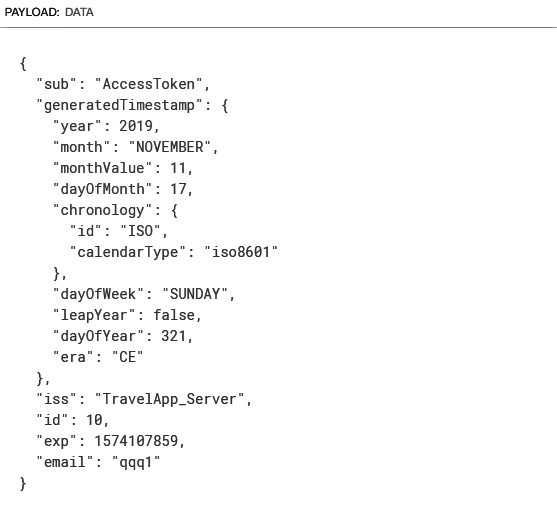
\includegraphics[width=\linewidth]{tokenPayload}
\caption{Rozszyfrowana zawartość podanego powyżej tokenu.}
\label{fig:tokenPayload2}
\end{figure}
\FloatBarrier


\section{Komunikacja z zewnętrznym API (Anna Malizjusz)}
\par Potrzeba wyszukiwania informacji o miejscach na świecie wymusiła korzystanie z zewnętrznych dostawców danych. Po analizie przeprowadzonej na etapie tworzenia specyfikacji wymagań systemowych zdecydowano o użyciu Here API \cite{Here}. Próba implementacji rozwiązania zmusiła programistów do skorzystania zarówno z wybranego dostawcy, jak i z początkowo odrzuconego Google API \cite{GoogleApi}, które oferowało dużo bogatszą bazę sposobów transportu.

\par Podstawowym problemem było odczytanie danych. Wynikiem wysłania zapytania do dostawcy informacji był ciąg znaków zawierający znaczą ilość danych nie tylko o temacie zapytania. W przypadku każdego typu żądania przeanalizowano wynik i zdefiniowane wspólną metodę wyszukującą oraz wybierającą niezbędne informacje. Następnie należało je dopasować do potrzeb -- nie wszystkie informacje były potrzebne aplikacji. Napisano funkcję zmieniającą ciąg znaków na instancję klasy. Skorzystano z możliwości klasy \textit{JsonParser} \cite{JsonParser} oraz \textit{GsonBuilder} \cite{GsonBuilder}.

\par Należało też uwzględnić sposób zapisanych informacji. Wiele znaków, np. "'" było zakodowanych, aby uniemożliwić wstrzykiwanie złośliwego kodu. W celu rozwiązania tego problemu skorzystano z funkcji \textit{StringEscapeUtils.unescapeHtml3()} \cite{escapeUtils}, która zmieniła formę znaków z kodowej na graficzną.

\section{Wspólne klasy serwera i aplikacji}
\par Podczas implementacji napotkano na problem powtarzających się klas w identycznej formie po stronie aplikacji i serwera. Stwarzało to kłopot przy edycji -- obie wersje pliku musiały być zawsze identyczne. Spróbowano rozwiązać to na następujące sposoby.

\subsection{Oddzielny projekt dodany jako moduł (Dorota Tomczak)}
\par Pierwszym pomysłem na wydzielenie wspólnych klas z projektu aplikacji i serwera było utworzenie osobnego projektu, który by te klasy zawierał. Następnie nowy projekt mógłby być dołączony jako moduł do obu projektów, co jednak okazało się być nietrywialnym rozwiązaniem między innymi ze względu na różnice w plikach gradle -- plik build.gradle w aplikacji mobilnej został napisany w języku Groovy, natomiast ten na serwerze w Kotlinie. Obie próby stworzenia takiego pliku dla wspólnego modułu w każdym ze wspomnianych języków nie powiodły się. Moduł mógł działać z określonym plikiem gradle tylko dla jednego z projektów jednocześnie. IDE, na którym otwarty był serwer podpowiadało, by usunąć wersję Kotlina w build.gradle, natomiast IDE aplikacji mobilnej podpowiadało wykonanie przeciwnej akcji. Po wielu próbach, ostatecznie porzucono zaproponowany pomysł na stworzenie osobnego projektu ze współdzielonymi klasami.

\subsection{Submoduły w repozytorium (Anna Malizjusz)}
\par Podjęto próbę dodania repozytorium zawierającego tylko wspólne pliki, a następnie wstawienia go do głównego repozytorium jako submoduły. Stworzyło to kolejne problemy w postaci konieczności częstych aktualizacji submodułów.
\par Zrezygnowano z submodułów i wykorzystano symboliczne powiązania.
Git traktował powiązany folder jako istniejący, więc nie powodowało to dodatkowych problemów. Plik zmieniony i zapisany w jednej z lokalizacji był automatycznie odwzorowywany w drugiej. Rozwiązanie to, choć z pozoru skuteczne nie mogło być wykorzystane przez wszystkich członków zespołu ze względu na różnice w systemie operacyjnym. Używane były zarówno komputery z system Windows, Linux oraz MacOS. Ostatecznie próby rozwiązania zarzucono.


\section{Rekomendacja miejsc z wykorzystaniem Collaborative Filtering (Dorota Tomczak)}
\par Po dodaniu elementu planu podróży można wejść w jego szczegóły i dokonać oceny miejsca, które znajduje się w planie. Oceny miejsc w skali od jednego do pięciu są przechowywane wraz z użytkownikami, którzy wystawili daną ocenę w osobnej tabeli bazy danych. Na podstawie tych ocen mogą być następnie obliczane rekomendacje przy użyciu techniki zwanej \textit{Collaborative Filtering}, a w szczególności jej odmianą opartą na użytkowniku (ang. user-based).
\par Do implementacji wspomnianej metody wyznaczania poleceń wykorzystano bibliotekę \textit{Apache Mahout} \cite{Apache Mahout}, która oferuje wiele implementacji algorytmów opartych o uczenie maszynowe. Po wskazaniu źródła danych, czyli w tym przypadku tabeli w bazie, utworzono model danych, który posłużył do wykonania niezbędnych obliczeń. Wyznaczenie polecanych miejsc przebiega w następujący sposób: wyliczane jest podobieństwo między użytkownikami algorytmem współczynnika korelacji Pearsona, algorytm k – najbliższych sąsiadów dla k równego 2 wyznacza najbardziej polecane miejsca, a na koniec na podstawie otrzymanych wyników tworzony jest obiekt klasy \textit{GenericUserBasedRecommender}. Wywołanie metody \textit{recommend} na obiekcie z podanym identyfikatorem użytkownika i liczbą rekomendacji, które ma zwrócić, skutkuje otrzymaniem listy identyfikatorów polecanych miejsc, jeśli zostały jakieś znalezione.
\par Testy przedstawionego rozwiązania aplikacją \textit{Postman} \cite{Postman} wykazały, że zwrócenie odpowiedzi trwa bardzo długo (nawet 20 s), a im większa liczba danych w bazie tym czas oczekiwania się wydłużał. Aby uniknąć konieczności oczekiwania na wynik po stronie aplikacji mobilnej, zdecydowano na prezentację polecanych miejsc w postaci powiadomień, czyli w momencie, gdy serwer jest gotowy na wysłanie rekomendacji wysyła odpowiednie powiadomienie, a do tego czasu użytkownik może dalej swobodnie nawigować po aplikacji.
\par W celu wysyłania powiadomień od serwera do aplikacji mobilnej skorzystano z usługi \textit{Firebase Cloud Messaging} \cite{Firebase}. Serwer po obliczeniu polecanych miejsc buduje wiadomość w postaci mapy, która ma zostać wysłana na urządzenie o określonym unikalnym tokenie. Za wysłanie odpowiada instancja klasy \textit{FirebaseMessaging}. W konsoli usługi można zobaczyć statystyki wysłanych wiadomości, które zawierają między innymi informacje o tym, ile z nich zostało otwartych przez użytkowników. Do odbierania wiadomości po stronie aplikacji mobilnej zaimplementowano serwis, który dzięki temu, że dziedziczy po \textit{FirebaseMessagingService} może reagować na zdarzenia takie jak nadejście wiadomości oraz zmiana tokena.
\par Gdy serwis odbierze wiadomość, odczytuje ją, a następnie tworzy powiadomienie, ustawiając jego parametry takie jak m.in. jego tytuł, priorytet, dźwięk. Powiadomienie jest następnie obsługiwane przez \textit{NotificationManager} i wyświetla się na ekranie urządzenia mobilnego. Użytkownik może powiadomienie od razu usunąć lub otworzyć. W drugim przypadku zostaje on przekierowany do aplikacji mobilnej, gdzie zostaje mu zaprezentowana lista polecanych miejsc wraz z nazwą i adresem.

\section{Dodawanie podróży (Magdalena Solecka)}
\par Podczas dodawania podróży tworzone są rekordy w dwóch tabelach bazy danych: \textit{travel} oraz \textit{app\_user\_travel}. Dodanie tylko jednego z nich powodowałoby zaśmiecanie bazy. W celu zapobiegnięcia takiej sytuacji wykorzystano transakcję (rys.~\ref{fig:travelTransaction}). Zmienna autocommit zostaje ustawiona na false, co jest równoznaczne z wymuszeniem manualnego wykonania operacji zapisu (ang. commit). Dodawane są kolejno dwa rekordy. W przypadku błędu zapisu do bazy wykonywana jest operacja cofnięcia operacji (ang. rollback). Jeżeli nie nastąpił żaden błąd wykonywana jest operacja zapisu (ang. commit), a zmiennej autocommit przepisywana jest z powrotem wartość true.

\begin{figure}[h]
\centering
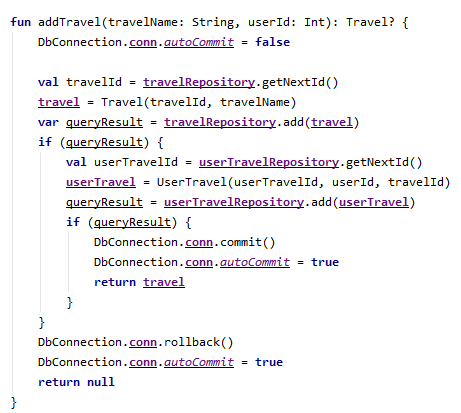
\includegraphics[width=\linewidth]{travelTransaction}
\caption{Transakcja dotycząca dodawania podróży.}
\label{fig:travelTransaction}
\end{figure}
\FloatBarrier

\section{Dostęp do bazy danych (Magdalena Solecka)}
\par Do implementacji połączenia z bazą został wykorzystany PostgreSQL JDBC Driver \cite{JDBC}. Zastosowano wzorzec Singleton, który w języku kotlin implementuje się używając słowa kluczowego \textit{object} zamiast \textit{class}.
\par Zaimplementowano również wzorzec repozytorium (ang. repository pattern). Opracowano bazowy interfejs generyczny IRepository oraz jego implementację Repository zawierające operacje typu CRUD -- podstawowe operacje dostępu do bazy danych takie jak dodawanie, usuwanie, odczyt i aktualizacja wiersza danych. Repozytoria dla poszczególnych modeli DAO (klas, których obiekty przechowują dane odczytywane z bazy) dziedziczą po generycznej klasie bazowej Repository (rys.~\ref{fig:repository}). Implementują również własny interfejs z funkcjami wymaganymi dla danej tabeli. Problemem przy wykorzystaniu typu generycznego okazało się tworzenie nowego obiektu, dlatego postanowiono wymusić na programistach implementację dodatkowej funkcji T tworzący ten obiekt dodając ją do interfejsu IRepository. W celu zmniejszenia ilości powtarzającego się kodu wyodrębniono również stałe fragmenty tekstu z zapytań SQL takie jak na przykład \textit{SELECT * FROM tableName } w postaci stałej selectStatement. Stałe zostały dodane do klasy bazowej Repository jako abstrakcyjne. W podobny sposób rozwiązano problem powtarzających się nazw tabel i kolumn. Nie udało się jednak utworzyć stałej abstrakcyjnej, wynikiem prób była pusta wartość w zapytaniach w miejscu gdzie powinna była znaleźć się na przykład nazwa tabeli.

\noindent\newline
\begin{figure}[h]
\centering
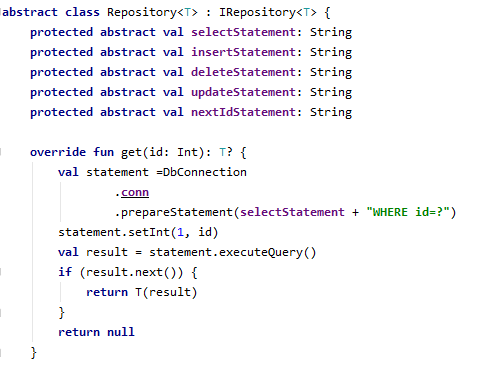
\includegraphics[width=\linewidth]{repository}
\caption{Klasa nadrzędna Repository.}
\label{fig:repository}
\end{figure}
\FloatBarrier